%%%%%%%%%%%%%%%%%%%% author.tex %%%%%%%%%%%%%%%%%%%%%%%%%%%%%%%%%
%
% sample root file for your "contribution" to a contributed volume
%
% Use this file as a template for your own input.
%
%%%%%%%%%%%%%%%% Springer Nature %%%%%%%%%%%%%%%%%%%%%%%%%%%%%%%%


% RECOMMENDED %%%%%%%%%%%%%%%%%%%%%%%%%%%%%%%%%%%%%%%%%%%%%%%%%%%
\documentclass[graybox]{SNmult}

%\usepackage{mathptmx}       % selects Times Roman as basic font
%\usepackage{helvet}         % selects Helvetica as sans-serif font
%\usepackage{courier}        % selects Courier as typewriter font
\usepackage{type1cm}        % activate if the above 3 fonts are
                            % not available on your system
%
\usepackage{makeidx}         % allows index generation
\usepackage{graphicx}        % standard LaTeX graphics tool
                             % when including figure files
\usepackage{multicol}        % used for the two-column index
\usepackage[bottom]{footmisc}% places footnotes at page bottom


\usepackage{newtxtext}       % 
\usepackage[varvw]{newtxmath}       % selects Times Roman as basic font
\usepackage{booktabs}        % publication-quality tables (toprule/midrule/bottomrule)
\usepackage{url}             % robust \url for bibliography URLs/DOIs with special chars
\usepackage{seqsplit}        % allow breaking of long typewriter identifiers in tables
\usepackage[bookmarks=true,bookmarksnumbered=true,colorlinks=false]{hyperref} % PDF bookmarks (load after url)
% Keep the title/author TOC entries out of the PDF outline (SNmult writes them
% to the TOC via \addcontentsline{toc}{title|author}; hyperref would otherwise
% turn them into top-level bookmarks).
\makeatletter
\providecommand*\toclevel@title{100}
\providecommand*\toclevel@author{100}
\makeatother

\makeindex             % used for the subject index
                       % please use the style svind.ist with
                       % your makeindex program

%%%%%%%%%%%%%%%%%%%%%%%%%%%%%%%%%%%%%%%%%%%%%%%%%%%%%%%%%%%%%%%%%%%%%%%%%%%%%%%%%%%%%%%%%

\begin{document}
% \motto{This is my motto.}       
% \title*{Quality-Controlled Synthetic SQuAD v2 Data for Extractive
%   Question Answering in Spanish Robbery Reports}
%   \titlerunning{Quality-Controlled Synthetic Data for Legal EQA}

\title*{A Proposed Methodology for LLM-Based Construction of a Synthetic
  SQuAD v2 Dataset for Fine-Tuning Extractive Question Answering in
  Spanish Robbery Reports}

% \titlerunning{Synthetic QA Dataset Construction and Transformer
% Fine-Tuning}
\titlerunning{LLM-Based  SQuAD Dataset Construction for
  EQA Fine-Tuning in Robbery Reports}
% Use \titlerunning{Short Title} for an abbreviated version of
% your contribution title if the original one is too long
\author{Lenin G. Falconi\orcidID{0000-0003-4402-6643} and\\
Myriam Hernandez-Alvarez\orcidID{0000-0003-4718-0400} and\\
Lorena Isabel Barona López\orcidID{0000-0002-5184-3759} and\\
Silvana Alexandra Arévalo-Carlosama\orcidID{0009-0004-0961-5850}}
\authorrunning{L. Falconi et al.}
\institute{Lenin G. Falconi \at Escuela Politécnica Nacional, Quito 170525, Ecuador, \email{lenin.falconi@epn.edu.ec}
\and Myriam Hernandez-Alvarez \at Escuela Politécnica Nacional, Quito 170525, Ecuador, \email{myriam.hernandez@epn.edu.ec}
\and Lorena Isabel Barona López \at Escuela Politécnica Nacional, Quito 170525, Ecuador, \email{lorena.barona@epn.edu.ec}
\and Silvana Alexandra Arévalo-Carlosama \at Instituto Superior Tecnológico de Tecnologías Inteligentes, Machachi 171110, Ecuador, \email{silvana.arevalo@instti.edu.ec}}
%
% Use the package "url.sty" to avoid
% problems with special characters
% used in your e-mail or web address
%
\maketitle
\abstract*{We propose an end-to-end methodology that uses open large language models to generate candidate SQuAD v2-style question--answer pairs from Spanish robbery narratives and represents unsupported information requests as explicit unanswerable instances. The methodology applies deterministic checks for schema conformance, literal answer support, answer-offset consistency, duplication, and answerability, followed by a stratified LLM-based semantic review designed to detect errors not visible through string matching alone. We evaluate the resulting dataset using context-disjoint splits and four pretrained extractive QA encoders in zero-shot and fine-tuned settings. Fine-tuning improves performance for the full-size models, with XLM-Roberta reaching a test F1 of 0.7801 and a reviewed-subset F1 of 0.6800. The results show that synthetic EQA data can support domain adaptation, but that structural validity alone does not establish semantic label reliability. We conclude with a reusable quality-control and review protocol for LLM-synthesized supervision in other under-resourced, sensitive-text domains.
\keywords{Extractive question answering $\cdot$ Legal NLP $\cdot$
  Synthetic data $\cdot$ SQuAD v2 $\cdot$ Large language models $\cdot$
  Dataset quality}}

\abstract{We propose an end-to-end methodology that uses open large language models to generate candidate SQuAD v2-style question--answer pairs from Spanish robbery narratives and represents unsupported information requests as explicit unanswerable instances. The methodology applies deterministic checks for schema conformance, literal answer support, answer-offset consistency, duplication, and answerability, followed by a stratified LLM-based semantic review designed to detect errors not visible through string matching alone. We evaluate the resulting dataset using context-disjoint splits and four pretrained extractive QA encoders in zero-shot and fine-tuned settings. Fine-tuning improves performance for the full-size models, with XLM-Roberta reaching a test F1 of 0.7801 and a reviewed-subset F1 of 0.6800. The results show that synthetic EQA data can support domain adaptation, but that structural validity alone does not establish semantic label reliability. We conclude with a reusable quality-control and review protocol for LLM-synthesized supervision in other under-resourced, sensitive-text domains.
\keywords{Extractive question answering $\cdot$ Legal NLP $\cdot$
  Synthetic data $\cdot$ SQuAD v2 $\cdot$ Large language models $\cdot$
  Dataset quality}}



\section{Introduction}
\label{sec:introduction}


Criminal reports contain relevant facts for law-enforcement and
judicial officials, but this information is usually embedded in
heterogeneous narrative descriptions. Relevant data such as where an
incident occurred, when it happened, which objects were stolen, and
what economic value was reported may appear alongside witness
accounts, procedural statements, contact information, vehicle
descriptions, and spelling inconsistencies. Given the high-volume
of robbery complains, it is of importance to develop systems that retrieve
evidence-supported facts from these documents that could reduce the effort
needed to review large collections of reports and support the work of
prosecutors.

Extractive question answering (EQA) is appropriate for this problem
because it constrains the output to a span from a provided
context. Given a question and a report, an EQA model predicts the
start and end positions of the answer in the original narrative. This
differs from generative question answering, whose output is composed
token by token and may not occur in the evidence. The extractive
constraint is valuable in legal and institutional settings: users can
inspect the textual basis of a returned answer rather than relying on
a fluent but potentially unsupported summary.

In our previous work, we investigated transformer-based EQA for
Spanish robbery reports from Ecuador. We used generative artificial
intelligence to construct a SQuAD-style dataset and evaluated a
Spanish BERT-based QA model in zero-shot and fine-tuned
settings. Fine-tuning improved the reported F1 score from 81.70 to
82.88, indicating that domain-specific supervision can improve fact
extraction from robbery narratives \cite{falconi2026robberyqa}. While
that work established the feasibility of the task, it also raised an
important methodological question: how reliable are the automatically
generated QA annotations used to train and evaluate the system?

This question matters whenever LLMs are used to construct
supervision. A generated answer can be fluent, syntactically valid,
and even occur literally in the source text while failing to answer
the intended question. A distance may be returned as a location, a
time associated with parking a vehicle may be confused with the time
of the robbery, or a generic phrase may be selected despite the
absence of an informative answer. Literal matching and a valid answer
offset are necessary for extractive QA data, but they are not
sufficient for semantic correctness.

The study is organized around four research questions:
\begin{itemize}
\item \textbf{RQ1.} Can open LLMs construct usable SQuAD v2-style EQA
  supervision from unlabeled Spanish robbery reports at scale, without
  per-example human authoring?
\item \textbf{RQ2.} Are literal-span validity and correct character
  offsets sufficient evidence that a generated question--answer pair
  is semantically correct, or is a further, independent review step
  required to detect errors that string matching cannot see?
\item \textbf{RQ3.} Does the constructed resource support effective
  extractive QA fine-tuning across encoder families and capacities,
  when evaluated under a leakage-free, context-disjoint protocol and
  against an independent, LLM-reviewed evaluation subset?
\item \textbf{RQ4.} Under a corrected, leakage-free evaluation
  protocol, does the original study's headline result still hold, and
  what specific factors, such as dataset composition, split methodology,
  and metric implementation, explain any discrepancy?
\end{itemize}

Compared with our previous work~\cite{falconi2026robberyqa}, this study
improves the construction and evaluation of synthetic EQA supervision: it
represents unsupported information requests as explicit unanswerable
instances, applies a reproducible quality-control pipeline to two open LLM
generators, and evaluates the resulting models under a leakage-free,
context-disjoint protocol. The main contributions of this study are therefore:
\begin{enumerate}
\item \textbf{An LLM-based methodology for synthetic SQuAD v2
    construction} from Spanish robbery narratives, producing
  answerable and unanswerable EQA instances with answer-span offsets
  and generator provenance.
\item \textbf{A reproducible quality-control protocol} (structural
  integrity $\rightarrow$ extractive validity $\rightarrow$ abstention
  consistency $\rightarrow$ span distribution/usefulness $\rightarrow$
  inter-generator agreement) that filters raw LLM output into
  \texttt{strict}, \texttt{expanded}, and \texttt{merged} dataset
  variants before any human or LLM review is needed.
\item \textbf{An LLM-based reviewer protocol for semantic reliability
    assessment}, using a second, independent LLM as a simulated
  annotator over a stratified sample, with an explicit error typology
  (wrong semantic type, wrong event reference, partial location,
  incomplete object list, answered-when-unanswerable, incorrect
  impossible, false abstention, other) and Wilson-score confidence
  intervals, explicitly distinguishing structural validity from
  semantic correctness.
\item \textbf{A leakage-aware evaluation protocol} using
  context-disjoint train/validation/test partitions and a held-out,
  LLM-reviewed evaluation subset, correcting the row-level,
  test-set-leaking split used in the original proof-of-concept study.
\item \textbf{A four-model extractive QA ablation} (two Spanish BETO
  variants, a multilingual XLM-Roberta model, and a distilled BETO
  model) comparing zero-shot and fine-tuned performance, including
  training-dynamics diagnostics (overfitting behavior, early stopping,
  no-answer threshold calibration) that the original study did not
  report.
\item \textbf{A direct, controlled replication of the original study's
    result}, run under the new codebase, that reproduces its headline
  number and then shows, on the same trained model, why that number
  does not hold under the new, harder, leakage-free
  benchmark, turning the original result into a diagnosed baseline
  rather than a competitor to be beaten.
\end{enumerate}

% Compared with our previous work~\cite{falconi2026robberyqa}, this study
% introduces three main changes. First, the annotation schema follows SQuAD v2,
% representing unsupported information requests as explicit unanswerable
% instances instead of the all-answerable SQuAD-style format used previously.
% Second, candidate annotations are generated by two open LLMs and passed through
% a deterministic quality-control pipeline rather than relying on a single
% unverified generator. Third, the evaluation protocol uses a context-disjoint
% split that prevents leakage between partitions, and the trained models are
% assessed on an LLM-reviewed evaluation subset rather than on the same generated
% labels used for training. These changes are evaluated through an ablation of
% four extractive QA encoders in zero-shot and fine-tuned settings.


The remainder of this paper is organized as follows. Section~\ref{sec:related-work}
introduces the foundational concepts and reviews the related literature on
legal NLP, LLM-based synthetic data generation, and the reliability of
LLM-generated annotations. Section~\ref{sec:methods} describes the proposed
methodology, including corpus characteristics, candidate generation, the
automatic quality-control protocol, the LLM-based semantic review, dataset
consolidation and splits, the extractive QA encoders, and the replication
design. Section~\ref{sec:results} reports the outcomes of the quality-control
pipeline, the semantic review, the fine-tuning ablation, and the original-study
replication. Section~\ref{sec:discussion} discusses the implications of these
findings. Section~\ref{sec:conclusion} concludes by answering the four
research questions and outlining directions for future work.

\section{Theoretical Background}
\label{sec:related-work}

\subsection{Foundational Concepts}
\label{sec:foundations}

\subsubsection{Language Models, Transformers, and Generative AI}

Transformer architectures use self-attention to learn context-dependent
representations and have become the foundation of modern language understanding
systems~\cite{vaswani2017attention}. Encoder models such as BERT can be adapted
to EQA by producing token representations from the combined question and
context and then estimating start and end distributions over the context
tokens~\cite{devlin2019bert}. The architecture is well suited to evidence-based
fact retrieval because it predicts positions in the original document rather
than freely generating an answer.

% ORIGINAL DEFINITION (kept commented for switching back):
% \begin{definition}[Generative artificial intelligence]
% Generative artificial intelligence (GAI) aims to learn a model distribution
% $p_{\mathrm{model}}(\mathbf{x})$ that approximates the true data distribution
% $p_{\mathrm{data}}(\mathbf{x})$:
% \begin{equation}
% p_{\mathrm{model}}(\mathbf{x}) \approx p_{\mathrm{data}}(\mathbf{x}),
% \label{eq:gai-def}
% \end{equation}
% where $\mathbf{x}$ represents observations from the data domain.
% \end{definition}
\begin{overview}{Generative artificial intelligence}
Generative artificial intelligence (GAI) aims to learn a model distribution
$p_{\mathrm{model}}(\mathbf{x})$ that approximates the true data distribution
$p_{\mathrm{data}}(\mathbf{x})$:
\begin{equation}
p_{\mathrm{model}}(\mathbf{x}) \approx p_{\mathrm{data}}(\mathbf{x}),
\label{eq:gai-def}
\end{equation}
where $\mathbf{x}$ represents observations from the data domain.
\end{overview}

% ORIGINAL DEFINITION (kept commented for switching back):
% \begin{definition}[Large language model]
% A large language model (LLM) defines a conditional probability distribution
% over the vocabulary $\mathcal{V}$ for the next token given a sequence
% $\mathbf{x}_{1:t} = (x_1, \ldots, x_t)$:
% \begin{equation}
% P(x_{t+1} \mid \mathbf{x}_{1:t}; \theta) = \mathrm{softmax}(\mathbf{W} \cdot \mathbf{h}_t + \mathbf{b}),
% \label{eq:llm-def}
% \end{equation}
% where $\theta$ denotes the model parameters and $\mathbf{h}_t$ is obtained by
% several layers of transformer blocks that process an embedded representation of
% the tokenized text:
% \begin{equation}
% \mathbf{h}_t = \mathrm{Transformer}(\mathbf{x}_{1:t}; \theta).
% \label{eq:h-def}
% \end{equation}
% \end{definition}
\begin{overview}{Large language model}
A large language model (LLM) defines a conditional probability distribution
over the vocabulary $\mathcal{V}$ for the next token given a sequence
$\mathbf{x}_{1:t} = (x_1, \ldots, x_t)$:
\begin{equation}
P(x_{t+1} \mid \mathbf{x}_{1:t}; \theta) = \mathrm{softmax}(\mathbf{W} \cdot \mathbf{h}_t + \mathbf{b}),
\label{eq:llm-def}
\end{equation}
where $\theta$ denotes the model parameters and $\mathbf{h}_t$ is obtained by
several layers of transformer blocks that process an embedded representation of
the tokenized text:
\begin{equation}
\mathbf{h}_t = \mathrm{Transformer}(\mathbf{x}_{1:t}; \theta).
\label{eq:h-def}
\end{equation}
\end{overview}

\subsubsection{Extractive Question Answering and the SQuAD v2 Task}

Question answering comprises tasks that differ in the evidence available to the
system and in the expected answer form. In open-domain QA, a system must
retrieve evidence from a large corpus. In reading-comprehension QA, the context
is provided alongside the question. EQA is a reading-comprehension formulation
in which the answer must be a contiguous span in the supplied context. Given a
tokenized context $C=(c_1,\ldots,c_n)$ and a question $Q$, an extractive reader
estimates a start and end position:
\begin{equation}
(s^*,e^*) = \arg\max_{1 \leq s \leq e \leq n} P(s,e\mid C,Q),
\label{eq:eqa}
\end{equation}
where the final answer is $c_{s^*:e^*}$. This formulation provides a direct
provenance relation: the answer is traceable to a particular segment of the
document.

The Stanford Question Answering Dataset (SQuAD) established a widely adopted
benchmark for extractive machine comprehension by pairing natural-language
questions with answer spans in Wikipedia passages~\cite{rajpurkar2016squad}.
SQuAD v2 expanded the task by adding adversarially written unanswerable
questions~\cite{rajpurkar2018know}. Thus, a model must decide not only which
span is relevant, but also whether the provided context contains evidence for
any answer. This selective-prediction property is particularly important in
robbery reports: a narrative may mention several times without stating the
robbery time, describe a location only vaguely, or omit a monetary value
altogether. Multilingual QA research confirms that extractive methods can be
evaluated beyond English; MLQA includes Spanish among its languages and
provides a benchmark for cross-lingual extractive QA~\cite{lewis2020mlqa}.
However, multilingual resources do not remove the need for domain-specific
data. Spanish robbery reports often contain informal grammar, regional
expressions, abbreviations, typographical errors, multiple events, and
ambiguous references, which motivates a domain-sensitive construction and
validation protocol.

\subsubsection{Zero-Shot and Transfer Learning}

Pretrained encoders can be evaluated zero-shot, i.e., without any additional
training on the target dataset, and then fine-tuned on domain supervision.
Zero-shot evaluation exposes the knowledge already present in the pretrained
checkpoint, whereas fine-tuning adapts the model to the target schema and
register at the risk of overfitting or catastrophic forgetting when the
training signal is noisy. Comparing both settings, as done in this study, makes
it possible to attribute performance gains to the dataset rather than to the
base model.

\subsubsection{LLMs as Synthetic Data Generators and Reviewers}

Two established uses of LLMs anchor this study. First, LLMs can act as
\textit{synthetic annotators} or generators of supervision. Answer-aware neural
question generation conditions a question on a designated answer within a
context, thereby strengthening question--answer alignment~\cite{zhou2017neuralqg};
position-aware generation further incorporates the answer's location in the
source text~\cite{sun2018answerfocused}. Second, LLMs can act as
\textit{automated judges or reviewers} that evaluate other models' outputs;
this LLM-as-judge paradigm has been formalized and benchmarked in the
literature~\cite{zheng2023judge}. The present study uses both roles: two LLMs
generate candidate SQuAD v2-style instances, and a third, independent LLM
reviews a stratified sample of those instances as a simulated annotator.

\subsection{Related Work}

% \subsubsection{Transformers in Legal and Evidence-Based NLP}

The legal domain presents specific challenges for NLP, including specialized
language, jurisdictional variation, long documents, incomplete standardization,
sensitive data, and limited expert annotations. Recent work surveying
transformer-based legal text processing documents the growing use of these
models for classification, retrieval, prediction, and question answering,
while stressing the importance of reliable task definitions and
evaluation~\cite{greco2024transformerlegal}. Legal NLP surveys likewise identify
data availability, interpretability, and transfer across legal systems as
central methodological concerns~\cite{niklaus2021legalnlp}.

Legal benchmarks have increased multilingual coverage, but coverage remains
uneven across jurisdictions and tasks. LEXTREME provides a multilingual and
multi-task legal benchmark, illustrating both the progress and the
fragmentation of legal NLP evaluation resources~\cite{niklaus2023lextreme}.
For Spanish, Legal-ES provides large-scale data for legal text processing from
legislative, administrative, and jurisprudential sources~\cite{gonzalez2020legales}.
Related work on legal information retrieval and entailment further motivates
traceable methods: Kim et al.\ apply transformer-based approaches to case-law
retrieval and legal entailment in the COLIEE setting~\cite{kim2024legalir}.
Although those tasks differ from short-span extraction, they share the
requirement that a system grounds its output in legal textual evidence, which
EQA provides through the predicted span.

% \subsubsection{LLM-Based Synthetic Data Generation for QA}

Beyond the legal benchmarks discussed above, large language models can produce
candidate labels, instructions, summaries, and QA pairs at a scale that is
difficult to achieve through exclusive manual annotation~\cite{zhou2017neuralqg,sun2018answerfocused}. This capability is
particularly valuable for low-resource domains such as Spanish criminal
narratives, where specialized annotation requires time and may be restricted by
data sensitivity. Recent legal QA research has also investigated the use of
LLM-generated supervision and distillation to produce legal QA
resources~\cite{italiani2025aceattorney}, which supports the practical value of
LLM-assisted data creation but increases the importance of transparent
validation. The study by Borroto et al.\ on question answering with LLMs and
learning from answer sets offers a related reliability perspective: it
illustrates the value of supplementing LLM processing with explicit and
externally checkable constraints~\cite{borroto2025llm2las}.

% \subsubsection{Quality Control and Reliability of LLM-Generated Data}

The reliability of such generated supervision, however, cannot be taken for
granted. Hallucination and unfaithfulness refer to generated content that is unsupported
by or inconsistent with the available evidence~\cite{ji2023hallucination,zhang2023siren}.
In synthetic EQA, a closely related failure can occur even if the answer string
appears in the report: the selected span can be semantically unrelated to the
requested information. A phrase such as ``a few meters away'' may be literal
but not a location; a time may refer to the discovery of theft rather than to
the robbery; and an isolated noun may omit other explicitly stolen items.
Evidence-based QA research emphasizes faithfulness, traceability, and
robustness as essential requirements for dependable LLM
systems~\cite{schimanski2024faithful}. These results motivate the two safeguards
central to this study: a deterministic quality-control pipeline for structural
and extractive validity, and an independent LLM-based semantic review for
residual semantic errors that string matching cannot detect.

% \subsection{Research Gap and Paper Positioning}

% The reviewed literature establishes that EQA provides an evidence-constrained
% prediction framework, that legal NLP requires domain-aware and multilingual
% evaluation, and that LLMs can scale synthetic data generation while creating
% faithfulness risks. The gap addressed in this research lies at their
% intersection. Existing work has not sufficiently characterized the semantic
% quality of LLM-generated SQuAD v2-style data for Spanish criminal-report EQA,
% and has not demonstrated whether such data, when quality-controlled and
% reviewed, supports trustworthy fine-tuning under a leakage-free protocol. This
% study therefore answers RQ1--RQ4 rather than only reporting a fine-tuned F1
% score: it evaluates whether the generated annotations themselves are reliable
% enough for training, whether a filtered and reviewed dataset produces more
% defensible results, and whether the original proof-of-concept result survives a
% corrected evaluation protocol.

\section{Materials and Methods}
\label{sec:methods}

This section describes the methodology followed for the extended
study. The pipeline comprises four stages: (i) construction of a SQuAD
v2-style dataset from Spanish robbery reports using open LLMs as
candidate generators; (ii) a deterministic automatic quality-control
(QC) stage, internally organised into five steps; (iii) a stratified LLM-based semantic review performed by an LLM
acting as an automated reviewer; and (iv) a leakage-free,
context-level evaluation protocol with zero-shot and fine-tuned
extractive QA models. Different to the previous approach
in~\cite{falconi2026robberyqa}, where only
\textsc{Llama}-3-8B-Instruct was used, we use two different open
instruction-tuned LLMs to generate the QA pairs. However, the text
preprocessing pipeline was inherited from the original
dataset. Consequently, texts used in this research are lowercase and
alphanumeric only. 

\subsection{Corpus Characteristics}

The study uses Spanish robbery reports from the Prosecutor's Office of
Ecuador, described in our prior work~\cite{falconi2026robberyqa}. The
corpus consists of 174594 reports of unlabeled narratives that
describe different incidents of robbery. These reports contain
sensitive information about the individuals involved, stolen items and
other characteristics of the robbery, such as location, time, and
value. Not all reports have the same information and statistical
analysis reported a mean of 112 words per report.

Each report is treated as one context. All QA instances
derived from the same report are assigned to the same partition by
their \texttt{context\_id}. This context-level partitioning prevents
leakage in which the training set contains one question from a report
while the test set contains another question derived from the same
narrative. However, the same incident may be reported by two different
individuals. This is something beyond the control of this research.

% Data governance is part of the methodology. The final version must state the
% legal basis for access, de-identification procedures, access restrictions,
% retention practices, and the conditions under which data or derived
% annotations can be shared. Where original reports cannot be released,
% reproducibility is supported through code, prompts, quality-control rules,
% model settings, and aggregate statistics.

\subsection{SQuAD v2-Style Candidate Generation}

Candidate QA pairs are generated from the robbery reports with two
open instruction-tuned LLMs:
\textsc{Gemma}-3-1B-IT~\cite{gemma3_1b_hf} and
\textsc{Qwen}-2.5-3B-Instruct~\cite{qwen2_5_3b_hf}. These two models
were selected because they are open-weight, are representative of two
different families and model sizes, and fit the available compute budget:
smaller models were deliberately preferred so that generation could run in
parallel across up to eight NVIDIA A16 GPUs with the required throughput,
rather than relying on a single larger model. Despite an effort to process the
174{,}594 reports in the corpus, given time and resource limits each model
processed the same 20{,}000-context sample and, for every context, received
the five target information questions shown in the original study (date, time,
place/address, stolen objects, and monetary value), producing up to
100{,}000 raw QA rows per generator.

The prompt requires a structured record with at least \texttt{context\_id},
\texttt{question}, \texttt{answer\_text}, \texttt{answer\_start},
\texttt{is\_impossible}, and generator provenance. When the document does not
explicitly support an answer, the model follows the controlled no-answer
protocol:
\begin{enumerate}
\item output the sentinel answer \texttt{ANSWER\_NOT\_FOUND};
\item set \texttt{is\_impossible=impossible}.
\end{enumerate}
Answerable rows must provide a literal span with its start offset. The
sentinel is later converted into a SQuAD v2 unanswerable row (empty answer,
\texttt{is\_impossible=true}), so the raw generation output remains traceable
while the final dataset follows the SQuAD v2 convention. Generation uses a
maximum of 512 new tokens, deterministic seeds, and a parallel multi-GPU
worker setup with resumable shards, as documented in the research
journal. Model identifiers, versions, inference software, quantization,
temperature, top-$p$, retries, and generation date are recorded for
reproducibility. The system prompt used for both generators asks the model to
extract literal, verifiable spans from the context and to abstain rather than
invent information:

% The system prompt is shown translated into English. The original Spanish
% prompt instructed the model to build a SQuAD-style dataset in Spanish;
% the literal sentinel emitted by the generator is RESPUESTA_NO_ENCONTRADA,
% rendered here as ANSWER_NOT_FOUND for consistency with the English text.
\begin{programcode}{System prompt (summarised, translated from Spanish)}
You are an assistant that extracts literal answers from a text to build\\
a SQuAD-style dataset in Spanish. Reply only with valid JSON.\\
If the context contains concrete information that answers the question, copy it\\
exactly as it appears:\\
\{"answer\_text": "exact text",\\
 "is\_impossible": "answered"\}.\\
If the context does not mention that information, do not invent or infer:\\
\{"answer\_text": "\seqsplit{ANSWER\_NOT\_FOUND}",\\
 "is\_impossible": "impossible"\}.\\
\end{programcode}
%% LLM-SOLVED

\subsection{Automatic Quality Control}

The automatic QC procedure is deterministic and precedes the semantic review.
It is organised in five internal steps: %that mirror the QC notebook (\texttt{qc\_squadv2\_datasets.ipynb}):

\begin{enumerate}
\item \textit{Structural integrity.} Each row must parse as JSON, contain the
  required fields, use valid labels, and be unique with respect to
  \texttt{(context\_id, question)}.
\item \textit{Extractive validity.} Generated offsets are never trusted: the
  \texttt{answer\_start}/\texttt{answer\_end} positions are recomputed against
  the context, and every answerable row must contain its
  \texttt{answer\_text} as a literal span of the context. Rows receive a
  transparent \texttt{qc\_status} label: \texttt{clean\_no\_answer},
  \texttt{empty\_no\_answer}, \texttt{free\_text\_no\_answer},
  \texttt{impossible\_but\_span\_present}, or
  \texttt{non\_extractive\_or\_hallucinated}. A row that fails literal-span
  verification is \emph{not} silently converted to ``impossible'': it is
  flagged as uncertain so that the distinction between a genuine abstention
  and a hallucinated answer is preserved.
\item \textit{Abstention consistency.} The sentinel and the
  \texttt{is\_impossible} label must be coherent, and answer versus abstention
  rates are measured globally and by question type.
\item \textit{Span distribution and usefulness.} Answer lengths, duplicate
  answers, and excessively long answers are analyzed; over-long answers are
  detected with a combined percentile and fixed-length rule.
\item \textit{Inter-generator agreement.} Because both generators processed the
  same \texttt{(context\_id, question)} pairs, their answerability and
  exact-answer agreement are compared directly.
\end{enumerate}

In addition to these structural checks, a context-aware semantic heuristic
flags candidates that may satisfy literal matching while posing semantic risk.
For locations, examples include deictic or non-informative spans such as ``the
indicated place'' or ``my home.'' For time questions, contexts with multiple
time references are flagged, especially when a time refers to a prior action,
discovery of the incident, or a period unrelated to the robbery. For object
questions, the pipeline flags obvious non-object answers and possibly
incomplete enumerations. For monetary values, it preserves currency
expressions where possible and flags contexts containing multiple
amounts.

The QC stage produces per-model strict and expanded SQuAD v2 variants, and a
merged dataset. The final merged corpus contains 80{,}726 rows (59{,}497
answerable and 21{,}229 unanswerable, approximately 27\% abstention), which is
the training corpus used in the experiments. Unanswerable rows are kept with
empty answers (standard SQuAD v2 abstention training), not dropped and not
filled with fake answers. This is an important improvement with
respect to our previous work in~\cite{falconi2026robberyqa}, which
only used answerable QA pairs. Of course, this makes our current goal
more challenging since the models are expected to recognize when the
context lacks of the answer to the provided question or the answer is
not literally written but can be understood by implication. The latter
is not considered for this study because of the definition of EQA.

Table~\ref{tab:abstention} summarises the answer and abstention behaviour of
each generator after QC, including the use of the controlled sentinel and free
text when the models abstained. Table~\ref{tab:agreement} reports the
inter-generator agreement over the 100{,}000 comparable pairs: the two models
agree on answerability in approximately 60\% of the cases and produce the same
exact answer in only about 25\% of the answered pairs, which motivates the
merged dataset rather than trusting a single generator. Figure~\ref{fig:span-gemma}
and Figure~\ref{fig:span-qwen} show the answer-span length distributions for
Gemma and Qwen, respectively, where the differences in response verbosity
between the two generators are visible.

% Source: out_qc_M2/table_abstention.tex
\begin{table}[!t]
\caption{Abstention consistency by model}
\label{tab:abstention}
\begin{tabular}{lrr}
\toprule
 & gemma & qwen \\
\midrule
answered & 56163.00 & 61340.00 \\
impossible & 43837.00 & 38660.00 \\
answer\_rate\_\% & 56.16 & 61.34 \\
abstention\_rate\_\% & 43.84 & 38.66 \\
consistent\_sentinel & 390.00 & 29008.00 \\
free\_text\_no\_answer & 43446.00 & 9619.00 \\
impossible\_but\_span\_present & 1.00 & 0.00 \\
\bottomrule
\end{tabular}
\end{table}

% Source: out_qc_M2/table_agreement.tex
\begin{table}[!t]
\caption{Inter-generator agreement}
\label{tab:agreement}
\begin{tabular}{lr}
\toprule
 & value \\
metric &  \\
\midrule
Comparable pairs & 100000.00 \\
Answerability agreement (\%) & 59.96 \\
Exact answer agreement among answered (\%) & 25.38 \\
No-answer agreement (\%) & 21.23 \\
Disagreement rate (\%) & 40.04 \\
\bottomrule
\end{tabular}
\end{table}

\begin{figure}[!t]
\centering
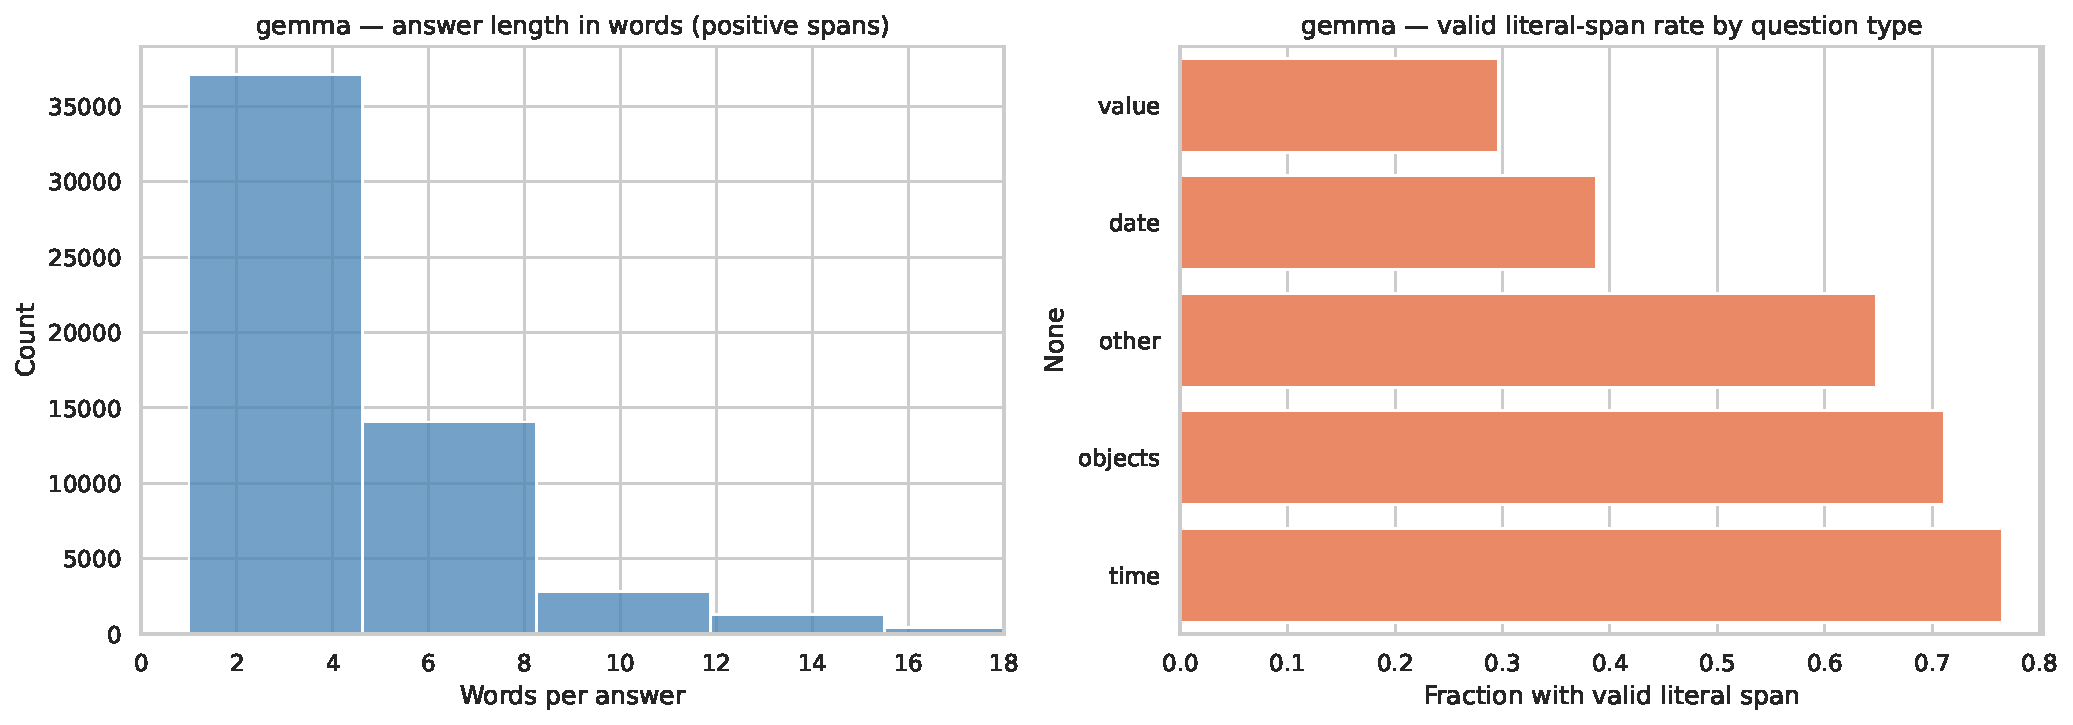
\includegraphics[width=\textwidth]{figures/span_distribution_gemma.pdf}
\caption{Answer-span length distribution for Gemma.}
\label{fig:span-gemma}
\end{figure}

\begin{figure}[!t]
\centering
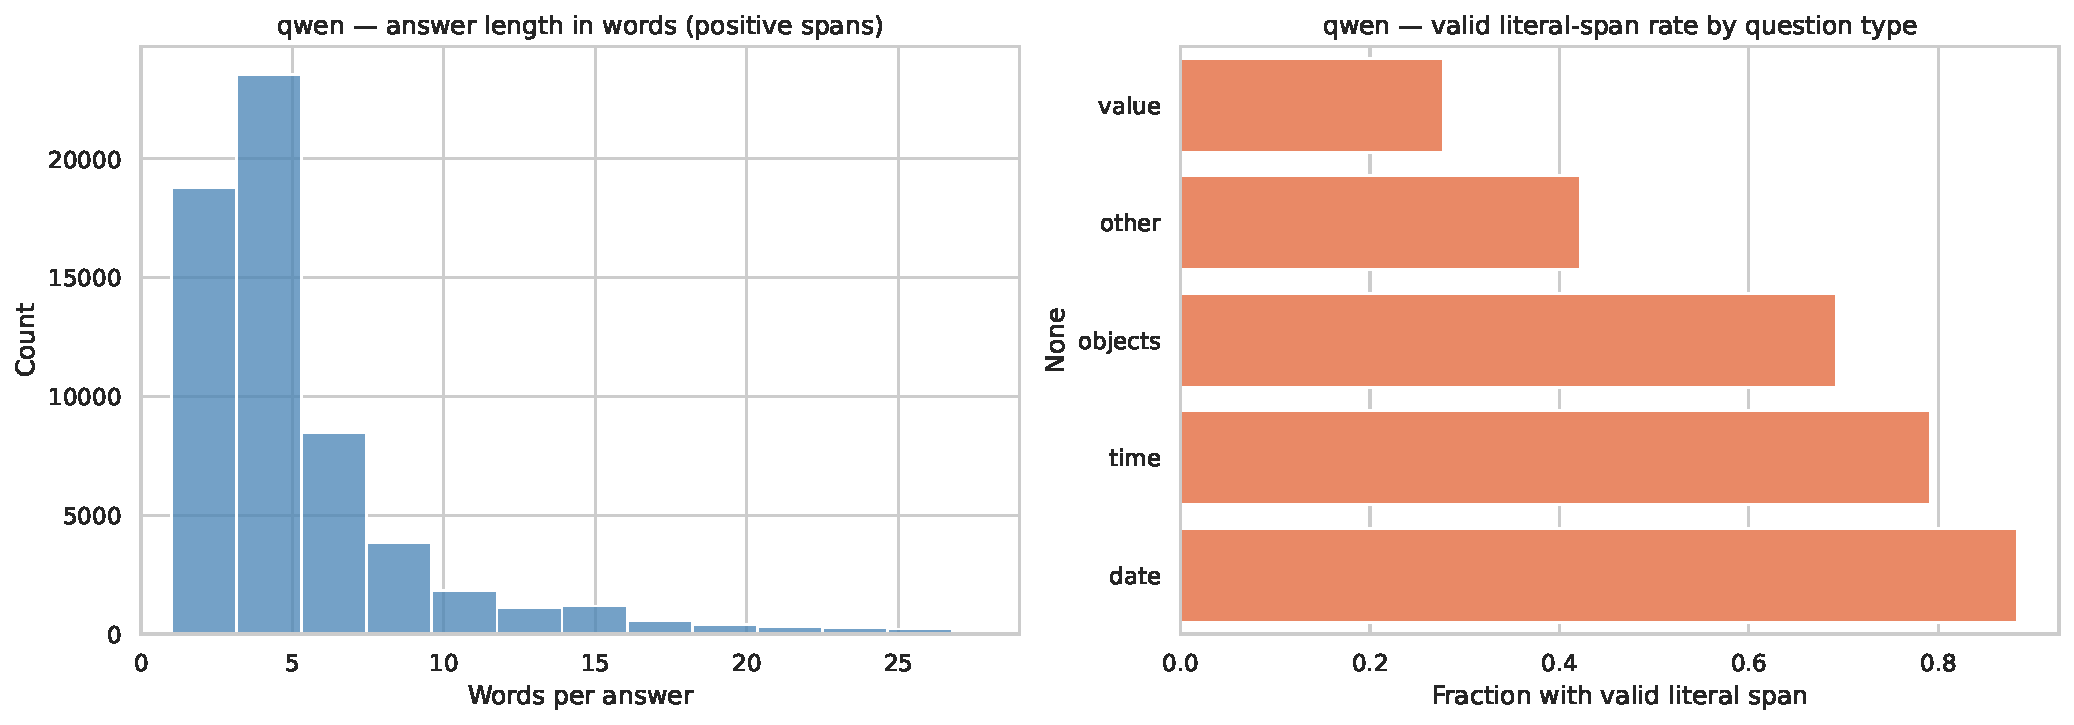
\includegraphics[width=\textwidth]{figures/span_distribution_qwen.pdf}
\caption{Answer-span length distribution for Qwen.}
\label{fig:span-qwen}
\end{figure}
%% LLM-SOLVED
\subsection{LLM-Based Semantic Review}

A stratified review sample of 200 rows (100 per generator) is drawn across
generating models, question categories, answerability labels, and QC statuses.
Each record is reviewed for semantic correctness, completeness, event
alignment, and correctness of the no-answer decision. The review is performed
by an LLM acting as an automated reviewer (Reviewer-LLM (R1), reviewer
id \texttt{R1})~\cite{glm45_techreport,glm_reviewer_hf}; no human intervention has
been carried out at this stage. The proposed error taxonomy is defined by the
following programming labels, each associated with a semantic concept:
\begin{enumerate}
\item \texttt{wrong\_semantic\_type}: the extracted span is literal but its
  semantic type does not match the requested information (e.g., a distance
  given as a location).
\item \texttt{wrong\_event\_reference}: the span belongs to a different event
  than the robbery (e.g., a time associated with parking the vehicle rather
  than with the incident).
\item \texttt{partial\_location}: the span is a valid but too vague or
  sub-specified location, even though the context provides a more precise one.
\item \texttt{incomplete\_object\_list}: the answer enumerates only part of the
  explicitly stolen objects.
\item \texttt{answered\_when\_unanswerable}: the model returns an answer even
  though the context does not support the requested information.
\item \texttt{incorrect\_impossible}: the model abstains although the context
  does contain a valid answer.
\item \texttt{false\_abstention}: the model labels an otherwise correct span as
  impossible.
\item \texttt{other}: any remaining semantic error not covered by the previous
  categories.
\end{enumerate}
%% LLM-SOLVED

The review is a statistically designed estimate of semantic label reliability
and a mechanism for improving automatic filters; it is not intended to
exhaustively label the entire corpus. The sample size of 200 rows was chosen so
that the observed correctness rates carry approximately $\pm 5$--7 percentage
point margins at 95\% confidence, balancing review cost against estimation
precision; Wilson score intervals are reported for the observed proportions.
Because the current review uses a single automated reviewer, inter-annotator
agreement metrics are not yet applicable. The 200 labeled rows constitute the
LLM-reviewed evaluation subset, which is held out and never used for training,
prompt revision, or hyperparameter selection.

\subsection{Dataset Versions and Splits}

The QC stage produces five immutable SQuAD v2 variants, all derived from the
same 20{,}000 contexts and the same five questions per context:

\begin{itemize}
\item \texttt{expanded\_gemma}: 99{,}999 rows (56{,}163 answerable and 43{,}836
  unanswerable); retains all parsed candidates, including 68 rows with invalid
  offsets.
\item \texttt{expanded\_qwen}: 100{,}000 rows (61{,}340 answerable and 38{,}660
  unanswerable); all rows are schema-valid.
\item \texttt{strict\_gemma}: 79{,}312 rows (35{,}476 answerable and 43{,}836
  unanswerable); drops answerable rows whose spans fail the recomputed offset
  check.
\item \texttt{strict\_qwen}: 85{,}042 rows (46{,}382 answerable and 38{,}660
  unanswerable); drops offset-invalid answerable rows.
\item \texttt{merged}: 80{,}726 rows (59{,}497 answerable and 21{,}229
  unanswerable, 26.3\% abstention); the model-agnostic training corpus used in
  the experiments.
\end{itemize}

Table~\ref{tab:readiness} summarises the SQuAD v2 readiness of these variants:
the merged corpus and both strict variants have zero schema errors, zero
invalid offsets, and zero duplicate identifiers, while \texttt{expanded\_gemma}
contains 68 rows with invalid offsets. This motivates the use of the merged
corpus as the training split rather than the raw expanded output.

% Source: out_qc_M2/analysis/table_squad2_readiness.tex
\begin{table}[!t]
\caption{SQuAD v2 readiness of the QC dataset variants.}
\label{tab:readiness}
\centering
\small
\begin{tabular}{lrrrrrr}
\toprule
Split & Rows & Answerable & Impossible & Impossible (\%) & Invalid offsets & Schema errors \\
\midrule
merged & 80{,}726 & 59{,}497 & 21{,}229 & 26.30 & 0 & 0 \\
strict\_gemma & 79{,}312 & 35{,}476 & 43{,}836 & 55.27 & 0 & 0 \\
strict\_qwen & 85{,}042 & 46{,}382 & 38{,}660 & 45.46 & 0 & 0 \\
expanded\_gemma & 99{,}999 & 56{,}163 & 43{,}836 & 43.84 & 68 & 68 \\
expanded\_qwen & 100{,}000 & 61{,}340 & 38{,}660 & 38.66 & 0 & 0 \\
\bottomrule
\end{tabular}
\end{table}

The final training partitions are obtained with a deterministic context-level
80/10/10 split (seed 42), so all experiment variants share the same partition.
The split is context-level rather than row-level because several questions
share the same source report: a row-level split would place sibling questions
from the same report in different partitions, leaking report-specific
information across train, validation, and test. The LLM-reviewed rows are
excluded from the partitions by \texttt{(context, question)} pair so that the
reviewed subset is never used as a design input and remains a held-out
evaluation set.
The resulting Hugging Face dataset
(\texttt{LeninGF/question-answering-robbery-m2}) contains 64{,}439 training
rows, 8{,}012 validation rows, 8{,}109 test rows, and 200 reviewer-labeled rows, all
in SQuAD v2 schema with \texttt{context\_id}.

\subsection{Models Used in This Research}
\label{sec:models}

This research relies on two groups of models: the LLMs used to generate and
review the SQuAD v2 dataset, and the extractive QA encoders evaluated in the
Option B ablation. To keep the text readable, each model is referred to by a
short name defined in Table~\ref{tab:model-reference}; the table also provides
the exact Hugging Face identifier and URL. Table~\ref{tab:model-summary}
summarises the main characteristics of these models.

\subsubsection{Models for SQuAD v2 Dataset Generation and Review}
\label{sec:models-generation}

The candidate QA pairs are generated with two open instruction-tuned LLMs:
Gemma-3-1B-IT~\cite{gemma3_1b_hf,gemma3_techreport} and
Qwen-2.5-3B-Instruct~\cite{qwen2_5_3b_hf,qwen2_5_techreport}
(Table~\ref{tab:model-reference}). Gemma-3-1B-IT is a compact multimodal model
from the Gemma 3 family; its 1B variant supports a context window of 32K
tokens and understands more than 140 languages, including Spanish.
Qwen-2.5-3B-Instruct is a dense decoder-only model from the Qwen2.5 family
with a 32K context window, multilingual support for over 29 languages, and a
training recipe optimised for instruction following. Both models are
open-weight, can run on the available GPU infrastructure, and are
representative of two different model families and sizes, which allows the
study to compare generator behaviour rather than relying on a single
annotation source.

The stratified LLM-based semantic review is performed by Reviewer-LLM (R1), an
LLM acting as an automated reviewer (reviewer id \texttt{R1})~\cite{glm45_techreport,glm_reviewer_hf,zeng2024chatglm}.
Reviewer-LLM is based on the GLM family of bilingual Chinese--English large
language models developed by Zhipu AI/Z.ai; the checkpoint used is
\texttt{zai-org/GLM-4.6}, whose model card points to the GLM-4.5 technical
report~\cite{glm45_techreport}. The family report describes models with
long-context support and tool-use capabilities that make them suitable for
structured annotation review.

\subsubsection{Models for the Extractive QA Ablation}
\label{sec:models-ablation}

The Option B ablation evaluates four pre-trained extractive QA encoders in
zero-shot and fine-tuned settings (Table~\ref{tab:model-reference}). The two
Spanish-only encoders are based on BETO~\cite{CaneteCFP2020}, a BERT model
pre-trained exclusively on Spanish data: mrm8488-BETO and
MMG-BETO~\cite{mrm8488_beto_squad2_hf,mmg_beto_squad2_hf}. Both follow the
BERT-base configuration (12 layers, 768 hidden units, 12 attention heads) and
were further fine-tuned on Spanish SQuAD-style data, giving them a maximum
sequence length of 512 tokens. The multilingual encoder is
XLM-Roberta~\cite{xlmr_squad2_hf,conneau2020xlmr}, based on XLM-Roberta, which
was pre-trained on 100 languages and fine-tuned on SQuAD 2.0. Finally, the
distilled encoder is Distilled-BETO~\cite{distill_beto_squad2_hf,sanh2019distilbert},
a Spanish BERT distilled with the DistilBERT approach, which retains a
512-token context but with a reduced number of layers and parameters.

% Source: Hugging Face model cards (URLs below); short names defined in this study.
\begin{table}[!t]
\caption{Short names, exact Hugging Face identifiers, and URLs of the models used in this research.}
\label{tab:model-reference}
\centering
\small
\begin{tabular}{p{3.0cm}p{4.4cm}p{3.2cm}}
\toprule
Short name & Hugging Face identifier & URL \\
\midrule
Gemma-3-1B-IT & \texttt{google/gemma-3-1b-it} & \seqsplit{https://huggingface.co/google/gemma-3-1b-it} \\
Qwen-2.5-3B-Instruct & \texttt{Qwen/Qwen2.5-3B-Instruct} & \seqsplit{https://huggingface.co/Qwen/Qwen2.5-3B-Instruct} \\
Reviewer-LLM (R1) & \texttt{zai-org/GLM-4.6} & \seqsplit{https://huggingface.co/zai-org/GLM-4.6} \\
mrm8488-BETO & \seqsplit{\texttt{mrm8488/bert-base-spanish-wwm-cased-finetuned-spa-squad2-es}} & \seqsplit{https://huggingface.co/mrm8488/bert-base-spanish-wwm-cased-finetuned-spa-squad2-es} \\
MMG-BETO & \seqsplit{\texttt{MMG/bert-base-spanish-wwm-cased-finetuned-squad2-es}} & \seqsplit{https://huggingface.co/MMG/bert-base-spanish-wwm-cased-finetuned-squad2-es} \\
XLM-Roberta & \seqsplit{\texttt{deepset/xlm-roberta-base-squad2}} & \seqsplit{https://huggingface.co/deepset/xlm-roberta-base-squad2} \\
Distilled-BETO & \seqsplit{\texttt{mrm8488/distill-bert-base-spanish-wwm-cased-finetuned-spa-squad2-es}} & \seqsplit{https://huggingface.co/mrm8488/distill-bert-base-spanish-wwm-cased-finetuned-spa-squad2-es} \\
\bottomrule
\end{tabular}
\end{table}

\begin{table}[!t]
\caption{Summary of the main characteristics of the models used in this research.}
\label{tab:model-summary}
\centering
\small
\begin{tabular}{p{2.8cm}p{1.5cm}p{1.4cm}p{1.2cm}p{1.5cm}p{3.0cm}}
\toprule
Model & Context (tokens) & Multilingual & Spanish & EQA fine-tuned & Reported performance \\
\midrule
Gemma-3-1B-IT & 32K & Yes (140+) & Yes & No & Competitive small-model performance in the Gemma 3 report \\
Qwen-2.5-3B-Instruct & 32K (128K ext.) & Yes (29+) & Yes & No & Cost-effective 3B model competitive within its size \\
Reviewer-LLM (R1) & up to 128K & Yes (bilingual focus) & Limited & No & Rivals GPT-4 on general benchmarks (family report) \\
BETO (base) & 512 & No & Yes & -- & Outperforms mBERT on most GLUES tasks \\
mrm8488-BETO & 512 & No & Yes & Yes & Fine-tuned Spanish SQuAD checkpoint \\
MMG-BETO & 512 & No & Yes & Yes & Fine-tuned Spanish SQuAD checkpoint \\
XLM-Roberta & 512 & Yes (100) & Yes & Yes & +14.6 XNLI, +13 MLQA F1 vs mBERT \\
Distilled-BETO & 512 & No & Yes & Yes & Retains 97\% of BERT GLUE (DistilBERT) \\
\bottomrule
\end{tabular}
\end{table}


\subsection{Extractive QA Models and Fine-Tuning}

Four pre-trained extractive QA encoders are evaluated in zero-shot (ZSL) and
fine-tuned (FT) settings: a Spanish BERT (BETO) fine-tuned on SQuAD
es~\cite{mrm8488_beto_squad2_hf}, a second Spanish BERT SQuAD-es
checkpoint~\cite{mmg_beto_squad2_hf}, a multilingual XLM-Roberta SQuAD2
checkpoint~\cite{xlmr_squad2_hf}, and a distilled Spanish BERT SQuAD-es
checkpoint~\cite{distill_beto_squad2_hf}. All four models are evaluated on the
same test and reviewer-labeled splits, and none is treated as a privileged headline model.

Zero-shot evaluation applies the pre-trained checkpoint directly to the test
and reviewer-labeled sets. Fine-tuning adapts each checkpoint to the merged M2 training
corpus with a learning rate of \(2 \times 10^{-5}\), weight decay of 0.01,
maximum sequence length of 384 tokens with a stride of 128, an effective batch
size of 64 (32 per device with gradient accumulation 2), and FP16
training. A preliminary plateau experiment (documented in the research
journal) showed a textbook overfitting signature: train loss decreased
monotonically while evaluation loss increased almost monotonically over 50
epochs, and validation F1 peaked mid-training and then declined. The final
ablation therefore uses early stopping on validation F1 (patience 2--3), with
a useful epoch range of roughly 10--15 rather than a large fixed epoch count,
and the best checkpoint is selected on the held-out validation split, never on
the test set.

For SQuAD v2, each model must also decide whether a question is answerable. A
no-answer threshold is tuned on the validation split and then frozen and
applied to the test set. Plain F1 at threshold zero is reported as a lower
bound; the oracle best-F1 threshold computed on the test set is never reported
as a result.

\subsection{Evaluation Metrics}
\label{sec:eval-metrics}

The metrics used in this study are grouped into two sets: metrics that assess
the quality of the synthetic dataset and its semantic review, and metrics that
assess extractive QA performance. The first group is described in
Section~\ref{subsec:quality-metrics} and the second in
Section~\ref{subsec:eqa-metrics}.

\subsubsection{Quality-Check Metrics}
\label{subsec:quality-metrics}

The quality of the synthetic dataset is described through structural pass
rates, answer and abstention rates, and inter-generator agreement, which are
reported as percentages. For the LLM-based semantic review, the observed
correctness rate is a binomial proportion, and its uncertainty is quantified
with the Wilson score interval:
\begin{equation}
\frac{1}{1+\frac{z^2}{n}}\left(\hat{p} + \frac{z^2}{2n} \pm z
\sqrt{\frac{\hat{p}(1-\hat{p})}{n} + \frac{z^2}{4n^2}}\right),
\label{eq:wilson}
\end{equation}
where $\hat{p}$ is the observed proportion, $n$ the sample size, and $z$ the
standard normal quantile (1.96 for 95\% confidence).

\subsubsection{EQA Metrics}
\label{subsec:eqa-metrics}

Extractive QA performance follows SQuAD v2 conventions. Exact match (EM) and
token-level F1 are computed with the standard normalization, which lowercases
the text, removes punctuation, and collapses whitespace. Metrics are
disaggregated by answerability (HasAns and NoAns) and by question type (date,
time, place, objects, value).

\textbf{Exact match.} For a prediction $p$ and a reference answer $g$, EM is
defined as:
\begin{equation}
\mathrm{EM}(p,g) = \begin{cases}
1, & \mathrm{norm}(p) = \mathrm{norm}(g),\\
0, & \text{otherwise,}
\end{cases}
\label{eq:em}
\end{equation}
where $\mathrm{norm}(\cdot)$ applies the standard normalization.

\textbf{Token-level F1.} Token-level F1 measures the overlap between the
predicted and reference tokens:
\begin{equation}
\mathrm{F1}(p,g) = \frac{2\,P\,R}{P + R}, \qquad
P = \frac{|T_p \cap T_g|}{|T_p|}, \qquad
R = \frac{|T_p \cap T_g|}{|T_g|},
\label{eq:f1}
\end{equation}
where $T_p$ and $T_g$ denote the token sets of the prediction and the reference
answer, respectively. For multiple reference answers, the maximum F1 is used.

\textbf{HasAns and NoAns.} HasAns metrics are computed only over answerable
questions, and NoAns metrics only over unanswerable questions. A correct NoAns
prediction is one in which the model abstains (empty prediction), whereas a
correct HasAns prediction is one in which the predicted span matches the
reference span.

The no-answer threshold protocol is as follows. Plain F1 at threshold 0.0 is
reported as a conservative lower bound. The headline number is the F1 obtained
with the threshold frozen from the best validation epoch and then applied to
the test set. The oracle best-F1 threshold computed on the test set
(\texttt{best\_f1}) is a diagnostic upper bound only and is never reported as a
primary result. This protocol is deliberately more conservative than the one
used in the original study, where the test set itself was used to select the
best checkpoint.

\subsection{Replication Protocol}
\label{sec:paper-replication}

To isolate the effect of the new dataset and evaluation protocol from the
model and training methodology, the original ICA paper experiment is
replicated with the legacy all-answerable dataset
(\texttt{LeninGF/robos-question-answering}), its legacy schema, row-level
split, and original hyperparameters. This replication reproduces the reported
zero-shot and fine-tuned results and provides a direct comparison baseline for
the extended SQuAD v2 setup.

\section{Results}
\label{sec:results}

This section reports the empirical outcomes of the proposed methodology. It
begins with the results of the generation and automatic quality-control
stages, which describe the construction and structural reliability of the
synthetic dataset. It then presents the outcomes of the LLM-based semantic
review, which estimates the semantic reliability of the reviewed subset and
identifies the most frequent error categories. Next, it reports the
fine-tuning ablation of the four extractive QA encoders on the held-out test
and LLM-reviewed subsets. Finally, it presents the controlled replication of
the original study, which places the headline result of the previous work
under a corrected, leakage-free evaluation protocol.

\subsection{Generation and Automatic QC Outcomes}

Each generator processed 20{,}000 robbery-report contexts and received the
same five target questions per context, producing 100{,}000 raw candidate QA
pairs per model (200{,}000 in total). Table~\ref{tab:qc-results} summarises
the generation and QC metrics per generator. Both models achieved 100\%
completeness and 100\% structural validity: all rows parsed as JSON, all
required fields were present, and no duplicate \texttt{(context, question)}
pairs were observed. The main difference between generators lies in their
answer and abstention behaviour: Gemma answered 56.16\% of the questions and
abstained in 43.84\% of them, whereas Qwen answered 61.34\% and abstained in
38.66\%. The automatic literal-span verification confirmed that every
answerable row contains its answer text literally in the context, and the
recomputed offsets were valid in 56.09\% (Gemma) and 61.34\% (Qwen) of the
rows; the remaining rows correspond to clean abstentions.

% Source: out_qc_M2/table_metrics_summary.tex
\begin{table}[!t]
\caption{Generation and automatic quality-control metrics by generator.}
\label{tab:qc-results}
\centering
\small
\begin{tabular}{lrr}
\toprule
Measure & Gemma & Qwen \\
\midrule
Contexts processed & 20{,}000 & 20{,}000 \\
Questions per context & 5 & 5 \\
Expected pairs & 100{,}000 & 100{,}000 \\
Generated pairs & 100{,}000 & 100{,}000 \\
Completeness (\%) & 100.00 & 100.00 \\
Answer rate (\%) & 56.16 & 61.34 \\
Abstention rate (\%) & 43.84 & 38.66 \\
Literal-span valid (\%) & 56.16 & 61.34 \\
Provided offset valid (\%) & 56.09 & 61.34 \\
Non-extractive (\%) & 0.00 & 0.00 \\
Strict rows retained & 79{,}312 & 85{,}042 \\
Expanded rows retained & 99{,}999 & 100{,}000 \\
Heuristic semantic flags & 19{,}730 & 14{,}680 \\
Mean answer words & 3.98 & 5.74 \\
\bottomrule
\end{tabular}
\end{table}

The inter-generator analysis over the 100{,}000 comparable pairs confirms that
the two generators are complementary rather than redundant: they agree on
answerability in 59.96\% of the pairs and produce the same exact answer in
only 25.38\% of the pairs in which both models answer
(Table~\ref{tab:agreement}). This motivates the construction of the merged
corpus, which combines Gemma-preferred answerable rows, Qwen-preferred
answerable rows, and rows in which both models agree on abstention. The merged
corpus contains 80{,}726 rows (59{,}497 answerable and 21{,}229 unanswerable),
and, as reported in Table~\ref{tab:readiness}, it is SQuAD v2 ready with zero
schema errors, zero invalid offsets, and zero duplicate identifiers.

% Source: out_qc_M2/table_merged_composition.tex
\begin{table}[!t]
\caption{Composition of the merged dataset.}
\label{tab:merged-composition}
\centering
\small
\begin{tabular}{lr}
\toprule
Source & Records \\
\midrule
Gemma (preferred) & 37{,}434 \\
Qwen (preferred) & 22{,}063 \\
Both (no-answer agreement) & 21{,}229 \\
\bottomrule
\end{tabular}
\end{table}

Figure~\ref{fig:answer-length} shows the answer-length distribution of the
answerable rows in the merged corpus, and Figure~\ref{fig:answer-words-kind}
shows the number of words per answer by question type. Both figures support
the observation that Qwen tends to produce longer, more verbose answers than
Gemma, which is relevant for span extraction difficulty and for the semantic
risk of incomplete or over-specific answers.

% Source: out_qc_M2/analysis/fig_answer_length.pdf
\begin{figure}[!t]
\centering
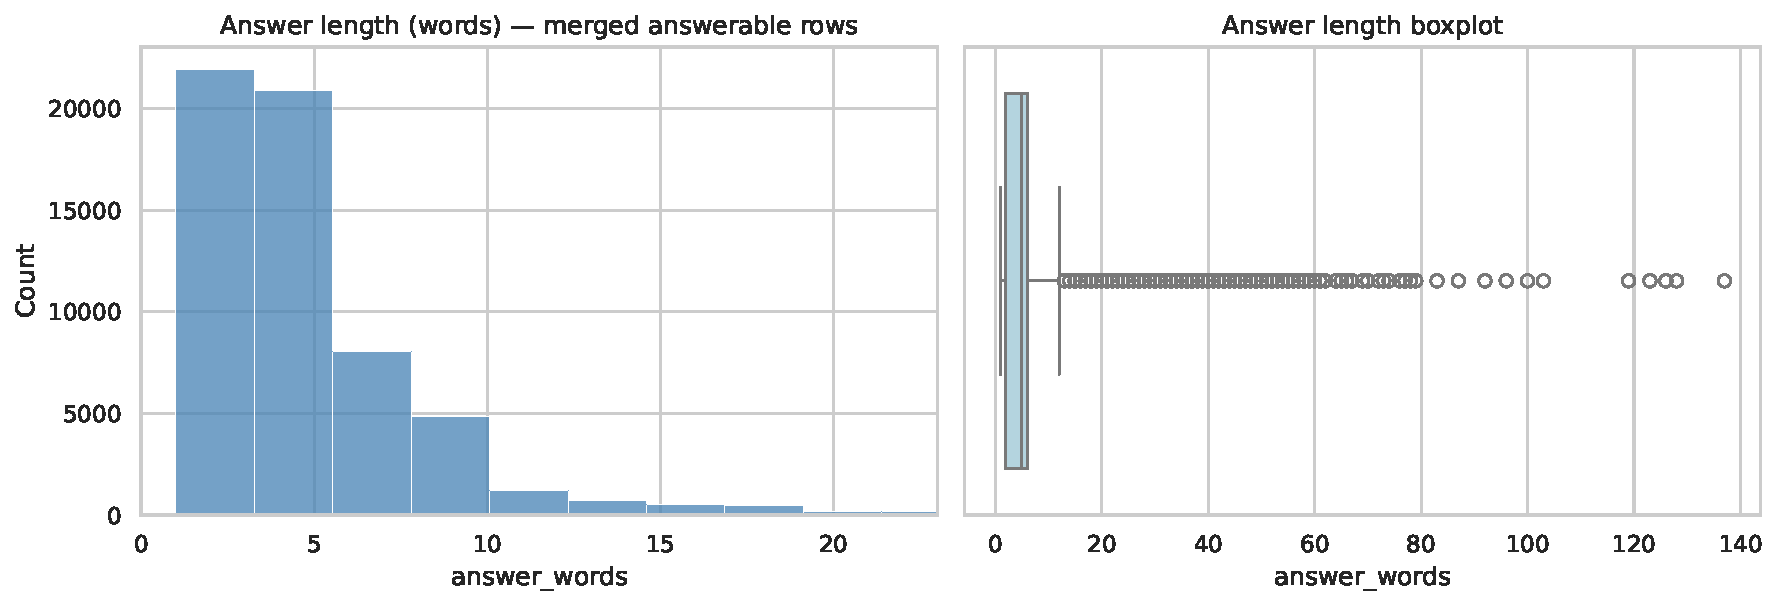
\includegraphics[width=\textwidth]{figures/answer_length_distribution.pdf}
\caption{Answer-length distribution of the answerable rows in the merged corpus.}
\label{fig:answer-length}
\end{figure}

% Source: out_qc_M2/analysis/fig_answer_words_by_kind.pdf
\begin{figure}[!t]
\centering
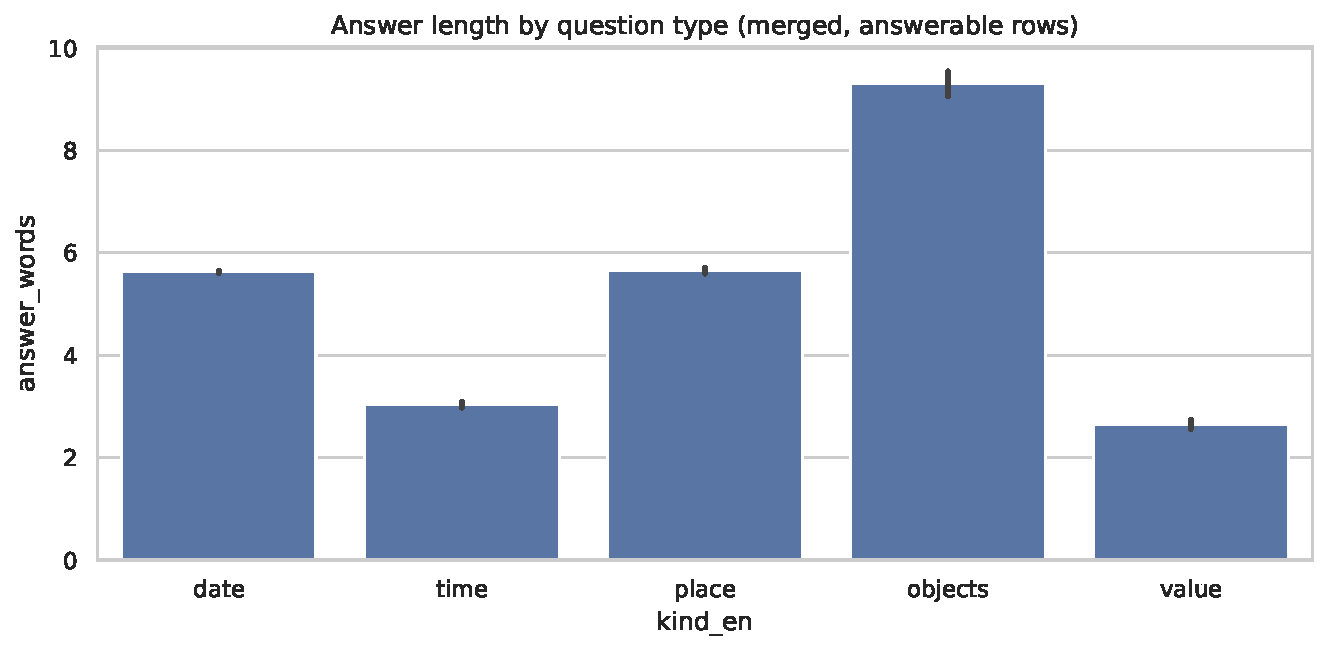
\includegraphics[width=\textwidth]{figures/answer_words_by_kind.pdf}
\caption{Number of words per answer by question type in the merged corpus.}
\label{fig:answer-words-kind}
\end{figure}

\subsection{Semantic Review Results}

Reviewer-LLM (R1) reviewed 200 stratified rows (100 per
generator). Table~\ref{tab:review-summary} reports the per-generator results:
Qwen obtained 73 correct rows (73.0\%, 95\% Wilson CI 0.636--0.807), while
Gemma obtained 57 correct rows (57.0\%, 95\% Wilson CI 0.472--0.663).
Figure~\ref{fig:review-accuracy-model} shows the same comparison graphically.
The review accuracy varies strongly by question type
(Table~\ref{tab:review-kinds}): Qwen is markedly more accurate on date
questions (95.8\%) but both models are weakest on place questions (Gemma
48.0\%, Qwen 47.1\%).

% Source: Reports/audit_glm_v1/outputs/table_audit_summary.tex
\begin{table}[!t]
\caption{Semantic review summary by generator model.}
\label{tab:review-summary}
\centering
\small
\begin{tabular}{lrrrr}
\toprule
Model & Reviewed $n$ & Correct & Incorrect & Accuracy \\
\midrule
Gemma & 100 & 57 & 43 & 0.570 \\
Qwen & 100 & 73 & 27 & 0.730 \\
\bottomrule
\end{tabular}
\end{table}

% Source: Reports/audit_glm_v1/outputs/fig_accuracy_by_model.pdf
\begin{figure}[!t]
\centering
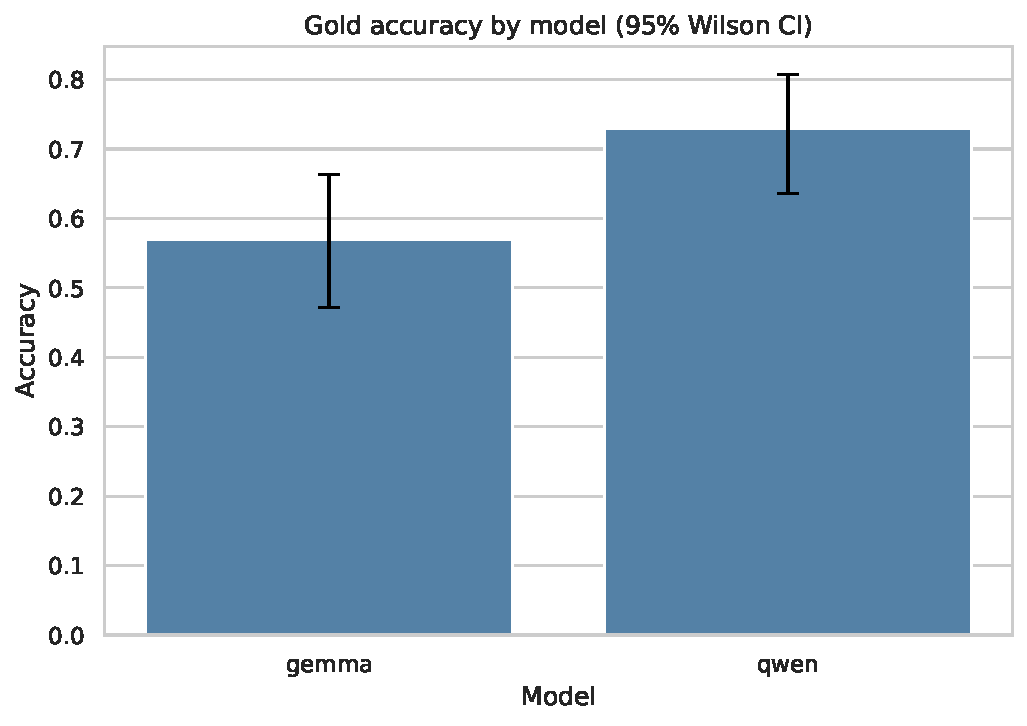
\includegraphics[width=0.85\textwidth]{figures/audit_accuracy_by_model.pdf}
\caption{GLM review accuracy by generator model (error bars show 95\% Wilson confidence intervals).}
\label{fig:review-accuracy-model}
\end{figure}

% Source: Reports/audit_glm_v1/outputs/table_audit_by_question_kind.tex
\begin{table}[!t]
\caption{Semantic review accuracy by question type and generator model.}
\label{tab:review-kinds}
\centering
\small
\begin{tabular}{llrrr}
\toprule
Model & Question type & Reviewed $n$ & Correct & Accuracy \\
\midrule
Gemma & date & 12 & 5 & 0.417 \\
Gemma & time & 24 & 14 & 0.583 \\
Gemma & place & 25 & 12 & 0.480 \\
Gemma & objects & 21 & 12 & 0.571 \\
Gemma & value & 18 & 14 & 0.778 \\
Qwen & date & 24 & 23 & 0.958 \\
Qwen & time & 26 & 19 & 0.731 \\
Qwen & place & 17 & 8 & 0.471 \\
Qwen & objects & 21 & 14 & 0.667 \\
Qwen & value & 12 & 9 & 0.750 \\
\bottomrule
\end{tabular}
\end{table}

The most frequent semantic errors are reported in
Table~\ref{tab:review-errors} and Figure~\ref{fig:review-error-types}.
False abstentions are the dominant failure mode (29 cases, 14.5\% of the
reviewed rows), followed by wrong time references (12 cases, 6.0\%) and
incomplete object lists (10 cases, 5.0\%). These categories confirm that
literal matching alone is insufficient: the extracted span may be valid in
string terms but semantically wrong, incomplete, or temporally misaligned.

% Source: Reports/audit_glm_v1/outputs/error_type_distribution.csv
\begin{table}[!t]
\caption{Distribution of semantic error types in the review sample.}
\label{tab:review-errors}
\centering
\small
\begin{tabular}{lrr}
\toprule
Error type & Count & Percentage \\
\midrule
None (correct) & 130 & 65.0 \\
false\_abstention & 29 & 14.5 \\
wrong\_time\_reference & 12 & 6.0 \\
incomplete\_object\_list & 10 & 5.0 \\
partial\_location & 6 & 3.0 \\
wrong\_semantic\_type & 4 & 2.0 \\
answered\_when\_unanswerable & 3 & 1.5 \\
non\_informative\_span & 3 & 1.5 \\
other & 3 & 1.5 \\
\bottomrule
\end{tabular}
\end{table}

% Source: Reports/audit_glm_v1/outputs/fig_error_type_distribution.pdf
\begin{figure}[!t]
\centering
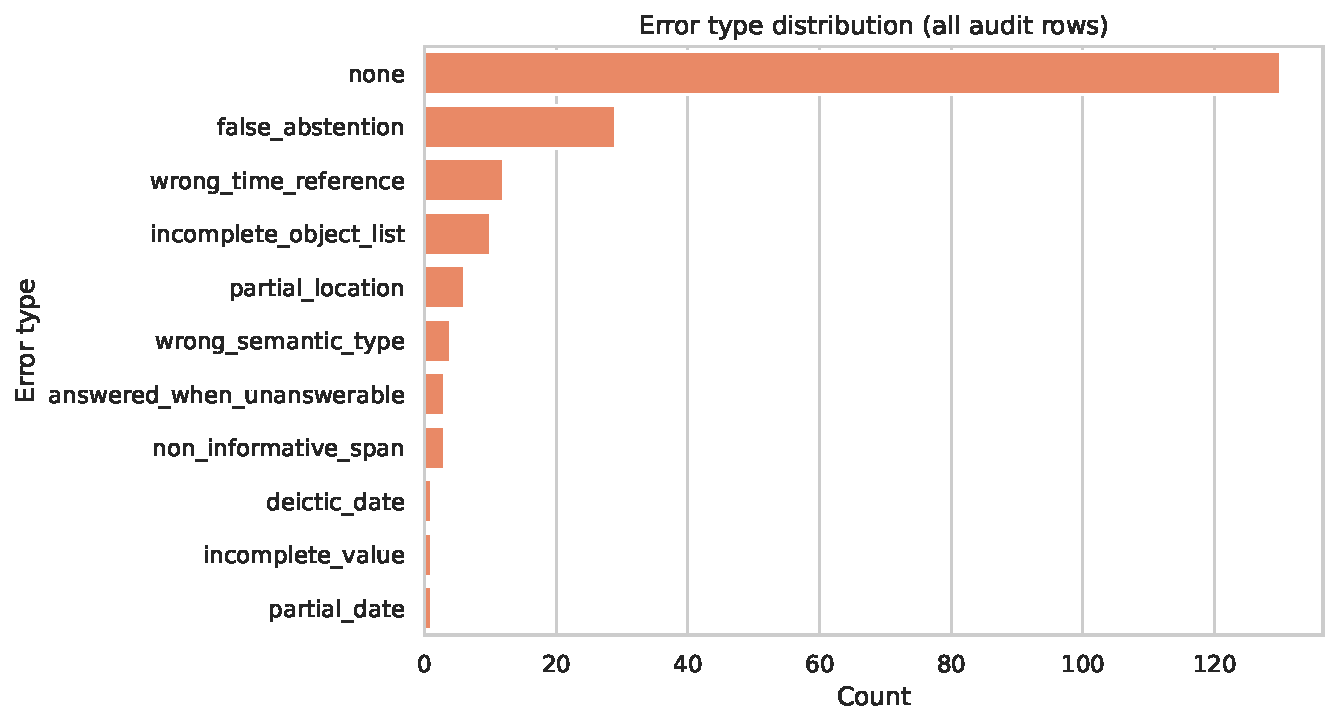
\includegraphics[width=0.9\textwidth]{figures/audit_error_type_distribution.pdf}
\caption{Distribution of semantic error types identified by the GLM automated reviewer.}
\label{fig:review-error-types}
\end{figure}

\subsection{EQA Evaluation on the LLM-Reviewed Subset}

The formal definitions of the EQA metrics (EM, token-level F1, HasAns/NoAns)
and the no-answer threshold protocol are given in
Section~\ref{sec:eval-metrics}. Table~\ref{tab:model-results} reports the
zero-shot (ZSL) and fine-tuned (FT) performance of the four extractive QA
encoders on the held-out test set (8{,}109 rows) and on the LLM-reviewed
subset (200 rows). Metrics are computed with the standard SQuAD v2
normalization and are reported as fractions; the no-answer threshold used for
the test set is the one tuned on the validation split and frozen before
evaluation. Figure~\ref{fig:ablation-comparison} provides a graphical
comparison of the same results.

Fine-tuning improves the overall token-level F1 on the test set for all four
models. The largest gains are obtained by the multilingual XLM-Roberta
checkpoint, whose test F1 increases from 0.6252 in the zero-shot setting to
0.7801 after fine-tuning, and by the MMG Spanish BERT checkpoint, which
improves from 0.6137 to 0.7484. The mrm8488 Spanish BERT checkpoint improves
from 0.6216 to 0.7272. The distilled checkpoint exhibits the weakest
performance in both settings, with a test F1 of 0.3844 in zero-shot and 0.3860
after fine-tuning, indicating that the reduced capacity of the distilled
encoder is insufficient for the SQuAD v2 task with abstention.

The same ordering is observed on the LLM-reviewed subset. Fine-tuning
raises the reviewed-subset F1 of deepset XLM-Roberta from 0.5093 to 0.6800 and that of
MMG-BETO from 0.5818 to 0.6627, whereas the gains for mrm8488-BETO are smaller
(0.5701 to 0.6074). For the distilled model, fine-tuning does not improve the
reviewed-subset F1 (0.3201 to 0.2836), which suggests that the distilled encoder does not
benefit from the additional training signal when the reference labels are
semantically reviewed rather than generated by the same process.

Table~\ref{tab:qtype-results} disaggregates the fine-tuned F1 by question
type. Date and monetary-value questions are consistently the easiest for all
models, whereas place and stolen-object questions remain the most difficult.
For the three non-distilled models, the fine-tuned place F1 ranges between
0.526 and 0.579 and the objects F1 between 0.558 and 0.623, which localizes
the main source of extraction error in spatial descriptions and in the
complete enumeration of stolen items. The distilled model performs poorly on
date, time, and place questions even after fine-tuning, and only reaches a
competitive F1 on the monetary-value category.

% Results aggregated with scripts/aggregate_results.py from
% out_experiments/option_b_abblation/ (per-experiment metrics_summary.json,
% gold_audit_metrics.json, and metrics_by_question_type.csv). All metrics are
% fractions; the test set has 8,109 rows and the LLM-reviewed subset 200 rows.
% Source: out_experiments/option_b_abblation/
\begin{table}[!t]
\caption{Zero-shot and fine-tuned EQA performance of the four encoders on the test and LLM-reviewed sets.}
\label{tab:model-results}
\centering
\small
\begin{tabular}{llrrrrrr}
\toprule
Model & Mode & Test EM & Test F1 & Test HasAns F1 & Test NoAns F1 & Reviewed EM & Reviewed F1 \\
\midrule
mrm8488-BETO & ZSL & 0.4158 & 0.6216 & 0.6013 & 0.6768 & 0.3450 & 0.5701 \\
mrm8488-BETO & FT & 0.5581 & 0.7272 & 0.6934 & 0.8195 & 0.3900 & 0.6074 \\
MMG-BETO & ZSL & 0.4235 & 0.6137 & 0.5655 & 0.7454 & 0.3700 & 0.5818 \\
MMG-BETO & FT & 0.5757 & 0.7484 & 0.7372 & 0.7790 & 0.4100 & 0.6627 \\
XLM-Roberta & ZSL & 0.4521 & 0.6252 & 0.5342 & 0.8738 & 0.3300 & 0.5093 \\
XLM-Roberta & FT & 0.6124 & 0.7801 & 0.7888 & 0.7564 & 0.4350 & 0.6800 \\
Distilled-BETO & ZSL & 0.3232 & 0.3844 & 0.1849 & 0.9296 & 0.2450 & 0.3201 \\
Distilled-BETO & FT & 0.3553 & 0.3860 & 0.1670 & 0.9848 & 0.2400 & 0.2836 \\
\bottomrule
\end{tabular}
\end{table}

\begin{figure}[!t]
\centering
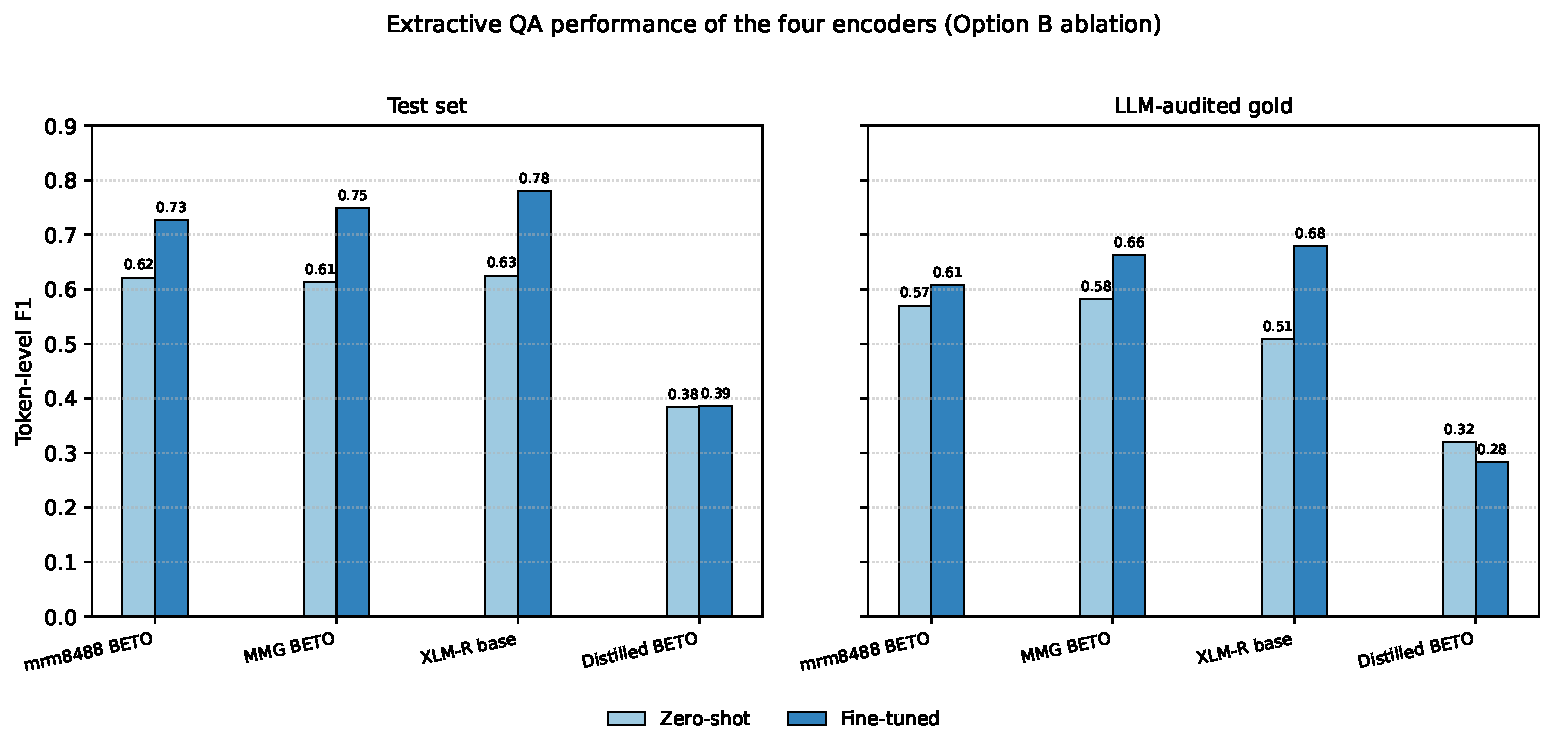
\includegraphics[width=\textwidth]{figures/ablation_model_comparison.pdf}
\caption{Comparison of zero-shot and fine-tuned token-level F1 of the four extractive QA encoders on the held-out test set (left) and on the LLM-reviewed subset (right).}
\label{fig:ablation-comparison}
\end{figure}

% Source: out_experiments/option_b_abblation/ (metrics_by_question_type.csv)
\begin{table}[!t]
\caption{Fine-tuned token-level F1 by question type for the four encoders.}
\label{tab:qtype-results}
\centering
\small
\begin{tabular}{lrrrrr}
\toprule
Model & Date & Time & Place & Objects & Value \\
\midrule
mrm8488-BETO & 0.896 & 0.734 & 0.526 & 0.558 & 0.836 \\
MMG-BETO & 0.919 & 0.743 & 0.554 & 0.576 & 0.859 \\
XLM-Roberta & 0.934 & 0.786 & 0.579 & 0.623 & 0.898 \\
Distilled-BETO & 0.199 & 0.314 & 0.286 & 0.336 & 0.745 \\
\bottomrule
\end{tabular}
\end{table}

\subsection{Comparison with the Original Study}

To separate the effect of the new dataset and evaluation protocol from the
model and training methodology, the original ICA experiment was replicated
with the legacy all-answerable dataset
(\texttt{LeninGF/robos-question-answering}), its legacy schema, row-level
split, and original hyperparameters (Section~\ref{sec:paper-replication}).
Table~\ref{tab:paper-replication} reports the replication results obtained
with the same Spanish BETO checkpoint used in the original study.

% Results aggregated with scripts/aggregate_results.py from
% out_experiments/paper_replication/ (metrics_summary.json and
% gold_audit_metrics.json). Test set = 457 legacy rows; reviewer-labeled = 200 M2 review rows.
\begin{table}[!t]
\caption{Comparison with the original study on the legacy all-answerable dataset.}
\label{tab:paper-replication}
\centering
\small
\begin{tabular}{lrrrr}
\toprule
Setting & EM & F1 & $n$ & Notes \\
\midrule
Zero-shot (legacy) & 0.1488 & 0.5113 & 457 & All-answerable test rows \\
Fine-tuned (legacy) & 0.5208 & 0.7999 & 457 & All-answerable test rows \\
Fine-tuned on reviewer-labeled review & 0.2100 & 0.5925 & 200 & M2 LLM-reviewed rows \\
\bottomrule
\end{tabular}
\end{table}

The fine-tuned replication reaches a token-level F1 of 0.7999 on the legacy
test split, closely matching the previously reported F1 of 82.88 and
confirming that the model and training procedure are correctly reproduced. The
zero-shot baseline is substantially lower (EM 0.1488, F1 0.5113), as expected
for a model that was not fine-tuned on the target schema. When the same
legacy-trained model is evaluated on the M2 LLM-reviewed subset, its F1
drops to 0.5925, which is below every M2-fine-tuned encoder reported in
Table~\ref{tab:model-results}. This comparison highlights the additional
difficulty introduced by the SQuAD v2 abstention protocol and the semantically
reviewed labels.

\section{Discussion}
\label{sec:discussion}

This study addresses a central risk in LLM-assisted dataset construction: treating synthetic annotations as reliable once they satisfy a basic output format. The empirical analysis must distinguish structural validity, semantic validity, and downstream model accuracy. Structural validity means that an answer occurs in the context and that its offset is correct. Semantic validity means that the answer actually addresses the question, identifies the correct event, provides sufficient specificity, and correctly represents missing evidence. Downstream accuracy measures whether an EQA model retrieves correct evidence in previously unseen reports. These properties are related but not interchangeable.

The proposed workflow preserves the benefit of LLMs, namely the ability to generate large pools of candidate QA pairs from unlabeled documents, while adding controls appropriate for legal NLP. Automatic checks ensure reproducible minimum requirements. The semantic review quantifies residual error and identifies failure modes that can inform stricter filters and improved prompting. An LLM-reviewed evaluation subset prevents final performance claims from depending entirely on labels generated by the same process used to create training data.

EQA should be understood as a decision-support component rather than an autonomous legal system. Its advantage is traceability: each extracted answer can be shown with the source span and surrounding report context. Its limitations include ambiguous narrative text, incomplete reports, source-document errors, model uncertainty, jurisdictional variation, and the possibility of selecting a semantically incorrect but literal span. Practical systems should support abstention, source inspection, correction, logging, and professional oversight.

The controlled replication in Section~4.4 provides the clearest demonstration of why evaluation methodology matters. The original headline F1 of 82.88 is best understood as a proof-of-concept score on an easier setup rather than as an error: the original test set was all-answerable, the test set itself was used to select the best checkpoint, and the metric implementation computed start and end token predictions independently. Under the corrected, leakage-free, abstention-inclusive protocol, the same modeling approach scores lower, but the estimate is unbiased. Reporting the drop as a methodological finding, rather than as model underperformance, is the central evaluation contribution of this study.

We present a reusable methodology that turns unlabeled Spanish robbery narratives into LLM-generated, quality-controlled SQuAD v2 supervision, and we demonstrate across several transformer readers that fine-tuning can improve EQA while semantic review remains essential for credible evaluation. The lower scores observed in this more careful study, compared with the original proof of concept, are therefore not a regression in model capability but a direct consequence of a more demanding and more strict evaluation design. Unanswerable questions now contribute to the test set, the context-disjoint split prevents leakage between partitions, and the evaluation labels come from an independent LLM-based review rather than from the same generation process used to build the training corpus. Under these conditions, a score that is lower but unbiased is more informative for practitioners than a higher score obtained under easier conditions.

% \section{Threats to Validity and Responsible Use}
% \label{sec:validity}
% 
% \paragraph{Construct validity.} EM and F1 measure reference agreement but do not fully measure answer relevance, completeness, or event alignment. The semantic review complements these metrics.
% 
% \paragraph{Internal validity.} Multiple QA pairs derived from one robbery report can cause leakage if they are split independently. Partitioning by \texttt{context\_id} mitigates this risk. Generator versions, prompts, parameters, and retry policies must be preserved for reproducibility.
% 
% \paragraph{External validity.} Findings based on robbery reports from Ecuador may not transfer to other criminal offenses, jurisdictions, report templates, or Spanish varieties. Replication must use new context-disjoint material and, ideally, independent annotators.
% 
% \paragraph{Responsible use.} The reports may contain sensitive information. The final work must document de-identification, access restrictions, and permissible sharing. The system must not determine culpability, replace legal judgment, or be used without human verification of the returned evidence.

\section{Conclusion}
\label{sec:conclusion}

The results of this study provide evidence for each of the four research
questions. The generation stage confirmed that open LLMs can produce usable
SQuAD v2-style supervision from unlabeled Spanish robbery reports at scale: two
open models generated 100{,}000 candidate rows per generator from 20{,}000
contexts with complete structural conformance, and the quality-control pipeline
reduced these candidates into five reproducible dataset variants, including an
80{,}726-row merged corpus. At the same time, the semantic review demonstrated
that structural validity does not guarantee semantic correctness:
approximately one third of the reviewed rows were semantically incorrect
despite passing the deterministic checks, with false abstentions and wrong time
references as the dominant error categories. A literal span match is therefore
necessary but not sufficient for reliable synthetic EQA supervision.

The fine-tuning experiments further showed that the constructed resource
supports effective domain adaptation, although the gains depend on model
capacity: all four encoders improved after fine-tuning, with XLM-Roberta
reaching the highest test F1 of 0.7801 and a reviewed-subset F1 of 0.6800,
whereas the distilled encoder remained comparatively weak and place and object
questions were consistently the most difficult. The controlled replication
placed these results in perspective by showing that the original headline F1
does not survive a corrected, leakage-free protocol. The original all-answerable
test set, the use of the test split for model selection, and a metric
implementation gap explain the drop, turning the previous result into a
diagnosed baseline rather than a benchmark to be matched.

Taken together, these findings lead to the central conclusion of this study: a
literal string match and a correct character offset are necessary but not
sufficient conditions for reliable synthetic EQA supervision. The methodology
offers four portable artifacts that practitioners and future researchers can
reuse in other under-resourced or sensitive-text domains: the deterministic
quality-control pipeline, the LLM-based reviewer protocol with its error
typology, the context-disjoint split methodology, and the threshold-calibration
protocol. Future work should focus on the weakest question types (place and
objects), expand the reviewed sample toward approximately 385 rows for a
$\pm 5\%$ margin at 95\% confidence, and validate the reviewer itself against
human judgment on a small sub-sample, since the LLM-reviewed subset is not a
substitute for human-verified ground truth.

%



%
% \begin{acknowledgement}
% If you want to include acknowledgments of assistance and the like at the end of an individual chapter please use the \verb|acknowledgement| environment -- it will automatically be rendered in line with the preferred layout.
% \end{acknowledgement}
%
% \ethics{Competing Interests}{Please declare any competing interests
% in the context of your chapter. The following sentences can be regarded as examples.\newline
% This study was funded by [X] [grant number X].\newline
%  [Author A] has a received research grant from [Company W].\newline
%  [Author B] has received a speaker honorarium from [Company X] and owns stock in [Company~Y].\newline 
%  [Author C] is a member of [committee Z].\newline 
% The authors have no conflicts of interest to declare that are relevant to the content of this chapter.}

\eject

% \ethics{Ethics Approval}{If your chapter includes primary studies with humans please declare the adherence of ethical standards. Example text: This study was performed in line with the principles of the Declaration of Helsinki. Approval was granted by the Ethics Committee of University B (Date.../No. ...).\newline 
%  In addition, for human participants, authors are required to include a statement that informed consent (to participate and/or to publish) was obtained from individual participants or parents/guardians if the participant is minor or incapable.\newline
% If animals are studied, authors should make sure that the legal requirements or guidelines in the country and/or state or province for the care and use of animals have been followed or specify that no ethics approval was required.}

% \section*{Appendix}
% \addcontentsline{toc}{section}{Appendix}
% %
% %
% When placed at the end of a chapter or contribution (as opposed to at the end of the book), the numbering of tables, figures, and equations in the appendix section continues on from that in the main text. Hence please \textit{do not} use the \verb|appendix| command when writing an appendix at the end of your chapter or contribution. If there is only one the appendix is designated ``Appendix'', or ``Appendix 1'', or ``Appendix 2'', etc. if there is more than one.

% \begin{equation}
% a \times b = c
% \end{equation}

% References are managed with BibTeX from references.bib.
% Each reference is cited in the text with \cite{key}.
% spmpsci is the Springer numeric citation style for computer science.
\bibliographystyle{spmpsci}
\bibliography{references}
\end{document}

% ============================================================================
% STYLE REFERENCE -- FIGURES AND TABLES (kept commented for later use)
% ============================================================================
% \begin{figure}[t]
% \sidecaption[t]
% \includegraphics{figure}
% \Description{This is figure Alt-Text for Figure grg2.}
% \caption{If the width of the figure is less than 7.8 cm use the \texttt{sidecaption} command to flush the caption on the left side of the page. If the figure is positioned at the top of the page, align the sidecaption with the top of the figure -- to achieve this you simply need to use the optional argument \texttt{[t]} with the \texttt{sidecaption} command}
% \label{fig:2}       % Give a unique label
% \end{figure}
%
% % Use the \index{} command to code your index words
% %
% % For tables use
% %
% \begin{table}[!t]
% \caption{Please write your table caption here}
% \label{tab:1}       % Give a unique label
% %
% % Follow this input for your own table layout
% %
% \begin{tabular}{p{2cm}p{2.4cm}p{2cm}p{4.9cm}}
% \hline\noalign{\smallskip}
% Classes & Subclass & Length & Action Mechanism  \\
% \noalign{\smallskip}\svhline\noalign{\smallskip}
% Translation & mRNA$^a$  & 22 (19--25) & Translation repression, mRNA cleavage\\
% Translation & mRNA cleavage & 21 & mRNA cleavage\\
% Translation & mRNA  & 21--22 & mRNA cleavage\\
% Translation & mRNA  & 24--26 & Histone and DNA Modification\\
% \noalign{\smallskip}\hline\noalign{\smallskip}
% \end{tabular}
% $^a$ Table foot note (with superscript)
% \end{table}
% ============================================================================

%%% Local Variables:
%%% mode: LaTeX
%%% TeX-master: t
%%% End:
